\documentclass[11pt, letterpaper]{article}
\usepackage[utf8]{inputenc}
\usepackage[letterpaper, margin=0.5in]{geometry}
\usepackage{amsmath}
\usepackage{amssymb}
\usepackage{amsthm}
\usepackage{graphicx}
\usepackage{listings}
\usepackage[font=scriptsize]{caption}
\usepackage{subcaption}
\usepackage{xcolor}
\graphicspath{ {.} }
\captionsetup{justification=raggedright, singlelinecheck=false}

\author{Ryan Tang}
\title{STA 602 HW 8}
\date{October 28th 2022}

\begin{document}
\maketitle

\section{Exercise 6.2}
\paragraph{(1) Glucose KDE}
The empirical distribution follows a "somewhat" normal shape. But it is skewed to the right.
\begin{figure*}[!h]
  \centering
  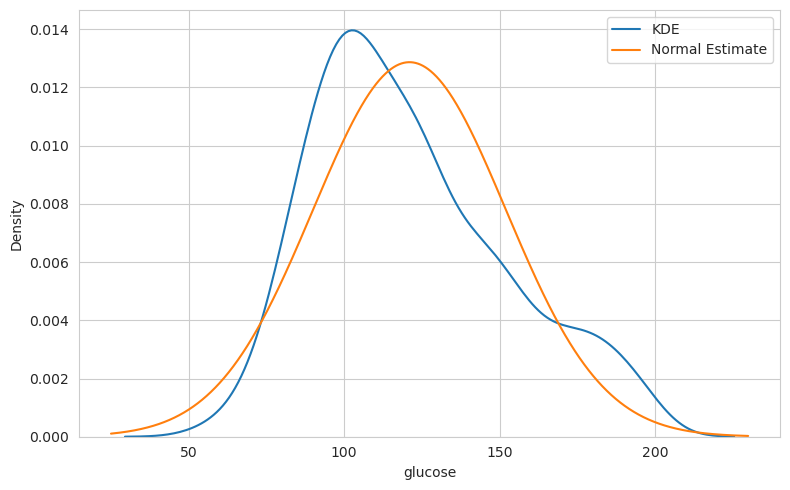
\includegraphics[width=0.7\textwidth]{6.2.1.png}
  \captionsetup{justification=centering}
  \caption{KDE vs Normal Assumption Comparison}
\end{figure*}

\paragraph{(2) Full conditionals}
We are given the following priors and hierarchical model.
\begin{align*}
    Y_i|X_i=k &\thicksim \mathcal{N}(\theta_k, \sigma^2_k) && k \in \{1, 2\} \\
    \theta_k &\thicksim \mathcal{N}(\mu_o, \tau_o^2) \\
    1/\sigma^2_k = \gamma_k &\thicksim Gamma(\frac{\nu_o}{2}, \frac{\nu_o\sigma_o^2}{2}) \\
    X_i &\thicksim Bernoulli(p) \\
    p &\thicksim Beta(a, b)
\end{align*}

Then we can write the following full conditionals regarding the joint in proportionality. And the full conditionals are decomposable in our setup. 
\begin{align*}
    N_k &= \sum_i^N \mathbb{I}(X_i=k) \\
    p(Y, \theta, \sigma^2, X, p) &= p(Y|\theta, \sigma^2, X, p) p(\theta|X,p) p(\sigma^2|X,p) p(X|p) p(p) \\
        &= p(p)
           \prod_i^{N_1} p(Y_i|\theta_1, \sigma^2_1)p(\theta_1)p(\sigma^2_1)p(X_i=1|p)
           \prod_i^{N_2} p(Y_i|\theta_2, \sigma^2_2)p(\theta_2)p(\sigma^2_2)p(X_i=2|p)
\end{align*}

In their full conditionals, $X_i$ and $p$ are still Bernoulli and Beta distributions.
\begin{align*}
    p(p|Y, \theta, \sigma^2, X) &\propto p(Y, \theta, \sigma^2, X, p) \\
        &\propto p(X|p)p(p) \\
        &\propto p^{a-1}(1-p)^{b-1} p^{N_1}(1-p)^{N_2} \\
        &\propto p^{a+N_1-1}(1-p)^{b+N_2-1} \\
        &\thicksim Beta(a+N_1, b+N_2) \\ \\
    p(X|Y, \theta, \sigma^2, p) &\propto \prod_i^N p(Y_i|\theta, \sigma^2, X_i, p) p(X_i|p) \\
        &\propto \prod_i^N
            \left[p(Y_i|\theta_1, \sigma^2_1) p(X_i=1|p)\right]^{\mathbb{I}(X_i=1)}
            \left[p(Y_i|\theta_2, \sigma^2_2) p(X_i=2|p)\right]^{\mathbb{I}(X_i=2)} \\
    p(X_i=1|Y_i, \theta, \sigma^2, p) &\propto p(Y_i|\theta_1, \sigma^2_1) p \\
        &\thicksim Bernoulli\left(
            p_1 = 
            \frac{\mathcal{N}(Y_i|\theta_1, \sigma^2_1) p}
                 {\mathcal{N}(Y_i|\theta_1, \sigma^2_1) p + \mathcal{N}(Y_i|\theta_2, \sigma^2_2) (1-p)}
        \right) \\
    p(X_i=2|Y_i, \theta, \sigma^2, p) &\propto p(Y_i|\theta_2, \sigma^2_2) (1-p) \\
        &\thicksim Bernoulli\left(
            p_2 = 
            \frac{\mathcal{N}(Y_i|\theta_2, \sigma^2_2) (1-p)}
                 {\mathcal{N}(Y_i|\theta_1, \sigma^2_1) p + \mathcal{N}(Y_i|\theta_2, \sigma^2_2) (1-p)}
        \right) \\
        &= 1 - p(X_i=1|Y_i, \theta, \sigma^2, p)
\end{align*}

$\theta_k$ and $\sigma_k$ are the normal semi-conjugate posterior forms in their full conditionals. However, the sufficient statistics are in terms of $N_1$ and $N_2$ that depend on the hidden $X$.
\begin{align*}
    p(\theta_1|Y, \sigma^2, X, p)
        &\propto p(\theta_1) \prod_i^{N_1} p(Y_i|\theta_1, \sigma^2_1) 
            && N_k \bar{Y}_k = \sum_i^N \mathbb{I}(X_i=k) Y_i \\
        &\thicksim \mathcal{N}(
            \mu_{N_1} = 
                \frac{\tilde{\tau}_o}{\tilde{\tau}_{N_1}} \mu_o + \frac{N_1\bar{Y_1}}{\tilde{\tau_{N_1}}}\gamma_1,
            \tilde{\tau}_{N_1} = \tilde{\tau_o} + N_1\gamma_1
        ) \\
    p(\theta_2|Y, \sigma^2, X, p)
        &\thicksim \mathcal{N}(
            \mu_{N_2} = 
                \frac{\tilde{\tau}_o}{\tilde{\tau}_{N_2}} \mu_o + \frac{N_2\bar{Y_2}}{\tilde{\tau_{N_2}}}\gamma_2,
            \tilde{\tau}_{N_2} = \tilde{\tau_o} + N_2\gamma_2
        ) \\
    p(1/\sigma_1^2|Y, \theta, X, p) &= p(\gamma_1|Y, \theta_1, X, p) \\
        &\thicksim Gamma(\frac{\nu_{N_1}}{2}, \frac{\nu_{N_1}\sigma_{N_1}^2}{2}) \\
        &\nu_{N_1} = \nu_o + N_1, \, \sigma_{N_1}^2 = \frac{1}{\nu_{N_1}}(\nu_o\sigma_o^2+\sum_{i\in N_1}(Y_i-\theta_1)^2) \\
    p(1/\sigma_2^2|Y, \theta, X, p) &= p(\gamma_2|Y, \theta_2, X, p) \\
        &\thicksim Gamma(\frac{\nu_{N_2}}{2}, \frac{\nu_{N_2}\sigma_{N_2}^2}{2}) \\
        &\nu_{N_2} = \nu_o + N_2, \, \sigma_{N_2}^2 = \frac{1}{\nu_{N_2}}(\nu_o\sigma_o^2+\sum_{i\in N_2}(Y_i-\theta_2)^2) \\
\end{align*}

\paragraph{(3) Gibbs Samples}


\section{Exercise 6.3}


\end{document}